\documentclass[aspectratio=169]{beamer}


%%%%%%%%%%%%%%%%%%%%%%%%%%%%%%%%%%%%%%%%%%%%%%%%%%%%%%%%%%%%%%%%%%%%%%%%%%%%%%%%%
% PREAMBLE

% DEFINE VARIABLES
\newcommand{\Lesson}{TEMA EJEMPLO}
\newcommand{\Subject}{Ejemplos, ejemplos, y ejemplos}
\newcommand{\Program}{Inversiones Financieras}
\newcommand{\Professor}{CUNEF Universidad}

% FOOTER WITH LOGO
\setbeamertemplate{footline}{
\hfill
\includegraphics[width=1.2cm]{figs/logo.png}\hspace{13cm}\vspace*{0.5cm}
\insertframenumber \hspace{1cm}
}

% FOOTER WITHOUT LOGO
\newcommand{\NoLogoFootline}{
    \setbeamertemplate{footline}{
    \hfill\vspace*{0.5cm}    
    }
}

% PACKAGES
\usepackage{framed, color}
\definecolor{shadecolor}{rgb}{1,0.9,0.8}
\usepackage[absolute,overlay]{textpos}
\usepackage{graphicx, tikz,xcolor}
\usepackage{multirow, bigstrut,epstopdf}
\usepackage{amsmath,relsize,bigdelim}
\usepackage{hyperref}
\hypersetup{
    colorlinks=true,
    linkcolor=blue,
    filecolor=magenta,      
    urlcolor=cyan,
}
\usepackage[font=tiny]{caption}

\setbeamercolor{block body}{bg=CUNEFGray!20,fg=Front}
\setbeamercolor{block title}{bg=CUNEFOrange,fg=white}



% IDENTATION OPTIONS
\setlength{\leftmargini}{1em} % for itemize and enumerate level 1
\setlength{\leftmarginii}{1em} % for itemize and enumerate level 2
\setlength{\leftmarginiii}{1em} % for itemize and enumerate level 3

% COLOR OPTIONS
\definecolor{CUNEFOrange}{RGB}{255, 87, 0}
\definecolor{CUNEFGray}{RGB}{214, 209, 196}
\definecolor{Front}{RGB}{21,31,108}
% BEAMER OPTIONS
\setbeamertemplate{navigation symbols}{}
\setbeamercolor{itemize item}{fg = CUNEFOrange}
\setbeamercolor{itemize subitem}{fg = CUNEFOrange}
\setbeamercolor{itemize subsubitem}{fg = CUNEFOrange}		
\setbeamercolor{enumerate item}{fg = CUNEFOrange}
\setbeamercolor{enumerate subitem}{fg = CUNEFOrange}
\setbeamercolor{enumerate subsubitem}{fg = CUNEFOrange}		
\setbeamercolor{normal text}{fg=Front}

\setbeamercolor{frametitle}{fg=CUNEFOrange}

% NEW TITLE SLIDE
\newcommand{\CUNEFTitleSlide}{\begin{frame}



%\begin{textblock*}{0.1\paperwidth}(0.01\paperwidth,0.01\paperwidth)
%\includegraphics[width=0.3\paperwidth]{Logo_WQU.png}
%\end{textblock*}

\vspace{2em}
%\centering\scriptsize{{\textcolor{CUNEFOrange}{\Lesson}}} \\[1em]
\centering\textbf{{\large\textcolor{CUNEFOrange}{Econometrics 2024/2025}}} \\ [1em]
\centering{\large\textcolor{CUNEFOrange}{}} \\ [1em]
\vspace{0.5em}
\centering{\normalsize\textcolor{CUNEFOrange}{Topic 0: Review of Statisics}}
\end{frame}}

% NEW SLIDE TEMPLATE
\newcommand{\slide}[2]{\begin{frame}
%\begin{textblock*}{0.1\paperwidth}(0.01\paperwidth,0.01\paperwidth)
%\includegraphics[width=0.15\paperwidth]{Logo_WQU.png}
%\end{textblock*}


\begin{textblock*}{0.87\paperwidth}(0.05\paperwidth,1.2cm)
{\Large\textcolor{CUNEFOrange}{#1}}
\end{textblock*}

\begin{textblock*}{0.87\paperwidth}(0.05\paperwidth,2cm)
#2
\end{textblock*}

\begin{textblock*}{\paperwidth}(0.01\paperwidth,0.95\paperheight)
\noindent\begin{tikzpicture}
%\draw[CUNEFOrange] (0,0) rectangle (0.9\paperwidth,0.8em);
%\draw[CUNEFOrange] (0.9\paperwidth+0.01\paperwidth,0) rectangle (\paperwidth-0.02\paperwidth,0.8em);
%\node[right] at (0,0.4em) {\tiny\textcolor{CUNEFGray}{\Subject\enspace-- \Program\enspace-- \Professor\enspace}};
\end{tikzpicture}
{\tiny\textcolor{CUNEFGray}\thepage}
\end{textblock*}
\end{frame}
}
%%%%%%%%%%%%%%%%%%%%%%%%%%%%%%%%%%%%%%%%%%%%%%%%%%%%%%%%%%%%%%%%%%%%%%%%%%%%%%%%%

% TOC AT BEGINNING OF EACH SECTION
\AtBeginSection[]{
    \begin{frame}<beamer>
    \frametitle{\textcolor{CUNEFOrange}{Outline}}
    \tableofcontents[currentsection]
    \end{frame}
}

\begin{document}

%%%%%%%%%%%%%%%%%%%%%
% Title Page
%%%%%%%%%%%%%%%%%%%%
\NoLogoFootline
{\usebackgroundtemplate{%
  
\includegraphics[width=\paperwidth,height=\paperheight]{figs/title_page.png}}
\CUNEFTitleSlide}

%%%%%%%%%%%%%%%%%%%%%
% Start slides
%%%%%%%%%%%%%%%%%%%%
\setbeamertemplate{footline}{
\hfill
\includegraphics[width=1.2cm]{figs/logo.png}\hspace{13cm}\vspace*{0.5cm}
\insertframenumber \hspace{1cm}
}

\begin{frame}
\frametitle{\textcolor{CUNEFOrange}{Outline}}
   \tableofcontents 
\end{frame}


\section{Mean, median and mode}
\frame<beamer>{\frametitle{\textcolor{CUNEFOrange}{Arithmetic Mean}}
\begin{itemize}
\item The \alert{arithmetic mean} (or simply mean) of a set of data is the sum of the data
values divided by the number of observations.
\item \alert{Population mean} (if we have the entire population available):
\begin{align*}
\mu = \frac{\sum_{i=1}^N x_i}{N}=\frac{x_1+x_2+\hdots+x_N}{N}
\end{align*}
where $\mu$ is the parameter.
\item If the data set is from a sample, then the \alert{sample mean} $\bar{x}$ is a statistic:
\begin{align*}
\bar{x} = \frac{\sum_{i=1}^N x_i}{N}=\frac{x_1+x_2+\hdots+x_N}{N}
\end{align*}
\item If the same observation repeats several times:
\begin{align*}
\sum_{i=1}^N x_i=\sum_{i=1}^N n_i\cdot x_i
\end{align*}
\end{itemize}
}


\frame<beamer>{\frametitle{\textcolor{CUNEFOrange}{Arithmetic Mean}}
\begin{itemize}
\item Arithmetic mean is the most intuitive and commonly used measure for central tendency.
\item It can be applied for \textbf{quantitative data only}. It is impossible to calculate arithmetic mean for qualitative data.
\item It has a major disadvantage: \alert{it is not robust to outliers}.
\end{itemize}
\alert{Robust:} strong, not-sensitive to small changes or variations.\\
\alert{Outlier:} atypical data point.
}

\frame<beamer>{\frametitle{\textcolor{CUNEFOrange}{Properties of the arithmetic mean}}


\begin{itemize}
\item Call $Y=a+b\cdot X$ a function of $X$, where $a$ and $b$ are some numbers.
\item Then we say that $Y$ is a \alert{linear} function of $X$.
\item If we know the mean of $X$, then the mean of $Y$ is just $\bar{y}=a+b\cdot \bar{x}$.
\end{itemize}
}

\frame<beamer>{\frametitle{\textcolor{CUNEFOrange}{Weighted mean}}
\begin{itemize}
\item Some situations require a special type of mean called a \alert{weighted mean}.
\item For example, in calculating the final grade for this course.
\item Or when we merge several groups together and want to calculate the overall mean.
\end{itemize}
\begin{align*}
W = \frac{\sum n_i x_i}{N}= \sum  w_i x_i,
\end{align*}
where $w_i=n_i/N$ and $\sum n_i=N$.
}

\frame<beamer>{\frametitle{\textcolor{CUNEFOrange}{Median}}
\begin{itemize}
\item The \alert{median} is the middle observation of a set of observations that are \textbf{ordered}
in increasing  order.
\item If the sample size, $n$, is an
even number, the median is the average of the two middle observations. 

\item The median can be found in 
$0.5(n + 1)th$ ordered position. If the position is with a decimal (like .5), take the mean of the two middle observations.
\item In many cases median is preferred because \alert{it is robust to outliers}.
\end{itemize}
}

\frame<beamer>{\frametitle{\textcolor{CUNEFOrange}{Mode}}
\begin{itemize}
\item The \alert{mode}, if one exists, is the most frequently occurring value. 
\item A distribution
with one mode is called unimodal; with two modes, it is called bimodal;
and with more than two modes, the distribution is said to be multimodal. 
\item The
mode is most commonly used with qualitative data.
\end{itemize}
}

\frame<beamer>{\frametitle{\textcolor{CUNEFOrange}{Mean, median, mode: the shape of the distribution}}
\begin{itemize}
\item Comparison of mean, median and mode also help to describe the shape of the distribution.
\end{itemize}
\begin{figure}
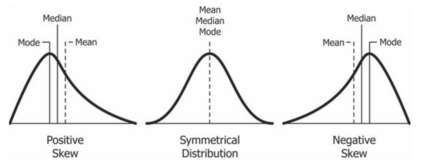
\includegraphics[width=0.7\textwidth]{figs/skew}
\end{figure}
}


\section{Variance and standard deviation}

\frame<beamer>{\frametitle{\textcolor{CUNEFOrange}{Variance and Standard Deviation}}
\begin{itemize}
\item The \alert{variance} is the
average of the sum of squared distances from the mean.

\item The \alert{population variance} $\sigma^2$ is the sum of the
squared differences between each observation and the \textit{population} mean
divided by the \textit{population} size $N$:
\begin{align*}
\sigma^2=\frac{\sum_{i=1}^N (x_i-\mu)^2}{N}
=\frac{\sum_{i=1}^N x_i^2}{N}-\mu^2
\end{align*}

\item The \alert{sample variance} \footnote{sometimes called a quasi-variance} $s^2$ is the sum of the
squared differences between each observation and the \textit{sample} mean
divided by the \textit{sample} size $N$ minus one:
\begin{align*}
s^2=\frac{\sum_{i=1}^N (x_i-\bar{x})^2}{N-1}=\frac{N}{N-1}\sigma^2
\end{align*}
\item To compute the variance requires squaring the distances, which then changes the
unit of measurement to square units. The standard deviation, which is the square root of
variance, restores the data to their original measurement unit.
\begin{align*}
\sigma = \sqrt{\sigma^2}\qquad s=\sqrt{s^2}
\end{align*}
\end{itemize}
}

\frame<beamer>{\frametitle{\textcolor{CUNEFOrange}{Variance and Standard Deviation: properties}}
\begin{itemize}
\item $\sigma^2$ and $\sigma$ are always $\geq$ 0
\item If $Y=a+b\cdot X$ and we know $\sigma^2_x$, then:
\begin{align*}
\sigma^2_y&= b^2 \cdot \sigma^2_x\\
\sigma_y&=\mid b  \mid\cdot \sigma_x\\
\end{align*}
\end{itemize}
}


\section{Covariance and correlation}

\frame<beamer>{\frametitle{\textcolor{CUNEFOrange}{Covariance}}
\begin{itemize}
\item \alert{Covariance}  is numerical a measure of the \textbf{linear} relationship between two variables.
\item A \alert{population covariance} is given by 
\begin{align*}
Cov(x,y)\equiv \sigma_{xy} = \frac{\sum_{i=1}^N (x_i-\mu_x)(y_i-\mu_y)}{N}=\frac{\sum x_i y_i}{N}-\mu_x\mu_y
\end{align*}

\item A \alert{sample covariance} is given by 
\begin{align*}
Cov(x,y)\equiv s_{xy} = \frac{\sum_{i=1}^N (x_i-\bar{x})(y_i-\bar{y})}{N-1}=\frac{N}{N-1}\sigma_{xy}
\end{align*}
\item If $s_{xy}>0$, then X and Y have a positive linear relationship; if  $s_{xy}<0$, then X and Y have a negative linear relationship; if $s_{xy}=0$, then X and Y do no have a linear relationship (might still have a non-linear relationship).
\item \textbf{Covariance  does not
provide a measure of the strength of the relationship}.
\end{itemize}
}


\frame<beamer>{\frametitle{\textcolor{CUNEFOrange}{Correlation}}
\begin{itemize}
\item A \alert{correlation coefficient} provides the direction (positive, negative) and strength (weak, moderate, strong).

\item A \alert{population correlation} coefficient:
\begin{align*}
\rho = \frac{\sigma_{xy}}{\sigma_x \sigma_y}
\end{align*}
\item A \alert{sample correlation} coefficient:
\begin{align*}
r = \frac{s_{xy}}{s_x s_y}
\end{align*}
\end{itemize}
}


\frame<beamer>{\frametitle{\textcolor{CUNEFOrange}{Correlation}}
\begin{itemize}
\item The correlation coefficient ranges from -1 to +1.
\item $r$ close to +1  indicates a positive \alert{linear}
relationship. 
\item $r$ close to -1 indicates a negative \alert{linear} relationship. 
\item When $r = 0$, there is no \alert{linear} relationship.
\end{itemize}
\begin{shaded}
If the two random variables are independent, the covariance/correlation will be zero. However, a covariance/correlation of zero does not necessarily mean that the variables are independent. A nonlinear relationship might exist.
\end{shaded}
}


\section{Regression line}


\frame<beamer>{\frametitle{\textcolor{CUNEFOrange}{Regression line}}
\begin{itemize}
\item Finally, we might want to \textbf{explain} the relationship between the two variables in economic terms. 
\item Also, we might want to \textbf{predict} the value of one variable given the value of another variable.
\item For example, if I know the number of views in CANVAS I can predict the student's grade.
\item For this we can draw a line through the scatterplot that \textbf{fits the data best}.
\item Such line is called a \alert{regression line}.
\end{itemize}
}


\frame<beamer>{\frametitle{\textcolor{CUNEFOrange}{Regression line}}
\begin{figure}
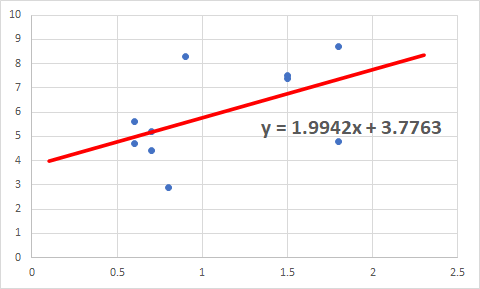
\includegraphics[scale=0.8]{figs/regression1}
\end{figure}
}


\frame<beamer>{\frametitle{\textcolor{CUNEFOrange}{Regression line}}
\begin{itemize}
\item In order to calculate the regression line, we have to calculate the slope and the intercept:
\begin{align*}
Y=a+b\cdot X,
\end{align*}
where $Y$ is the dependent variable and $X$ is the explanatory variable.
\item The slope and the intercept are given by:
\begin{align*}
b=\frac{\sigma_{xy}}{\sigma^2_x},\qquad a=\bar{y}-b\cdot \bar{x}
\end{align*}
\item The goodness of fit is measured by the \alert{coefficient of determination}:
\begin{align*}
R^2=r^2
\end{align*}
\end{itemize}
}


\frame<beamer>{\frametitle{\textcolor{CUNEFOrange}{Regression line}}
\begin{itemize}
\item The coefficients of the regression line can be interpreted as follows:
\begin{itemize}
\item[-] When $X$ increases (decreases) by one unit, $Y$ will increase (decrease) by $b$ units.
\item[-] When the value of $X$ is equal to zero, $Y$ will be equal to $a$.
\end{itemize}
\item Given the regression line, we can also make predictions by plugging in a value of $X$ into the equation.
\item $R^2$ varies from 0 to 1. $R^2$  measures the proportion of variation in the dependent variable ($Y$) that can be attributed to the independent variable ($X$). 
\begin{itemize}
\item[-] If $R^2$ is close to 0, then the goodness of fit is bad and the explanatory power of $X$ is low.
\item[-] If $R^2$ is close to 1, then the goodness of fit is good and the explanatory power of $X$ is high.
\end{itemize}

 
\end{itemize}
}


\frame<beamer>{\frametitle{\textcolor{CUNEFOrange}{Regression line: example}}
Consider investigating how years of education affect income.
\begin{itemize}
\item Which variable is the dependent variable $Y$?
\item Which variable is the explanatory variable $X$?
\item What relationship do you expect to find?

\end{itemize}
}

%
\frame<beamer>{\frametitle{\textcolor{CUNEFOrange}{Regression line: example}}
Now you collect some data about the years of education and monthly income of five people.
\begin{figure}
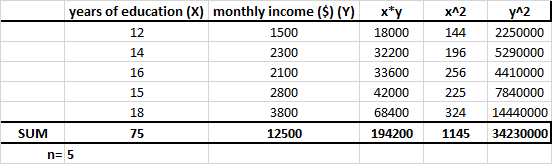
\includegraphics[scale=0.7]{figs/example2.png}
\end{figure}
\begin{itemize}
\item How does an increase in one year in education affect income?
\item What income would you predict for a person who has 17 years of education (12 years of high school + 5 years of double university degree)?
\item Evaluate the goodness of fit.
\end{itemize}
}




\frame<beamer>{\frametitle{\textcolor{CUNEFOrange}{Regression line: example}}

\begin{figure}
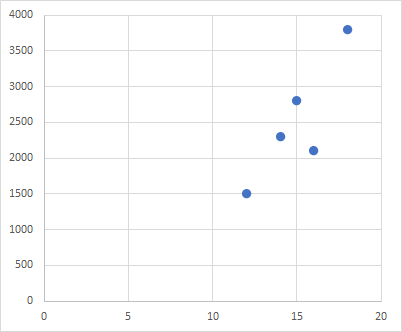
\includegraphics[scale=0.7]{figs/example3}
\end{figure}
}



\frame<beamer>{\frametitle{\textcolor{CUNEFOrange}{Regression line: example}}

\begin{figure}
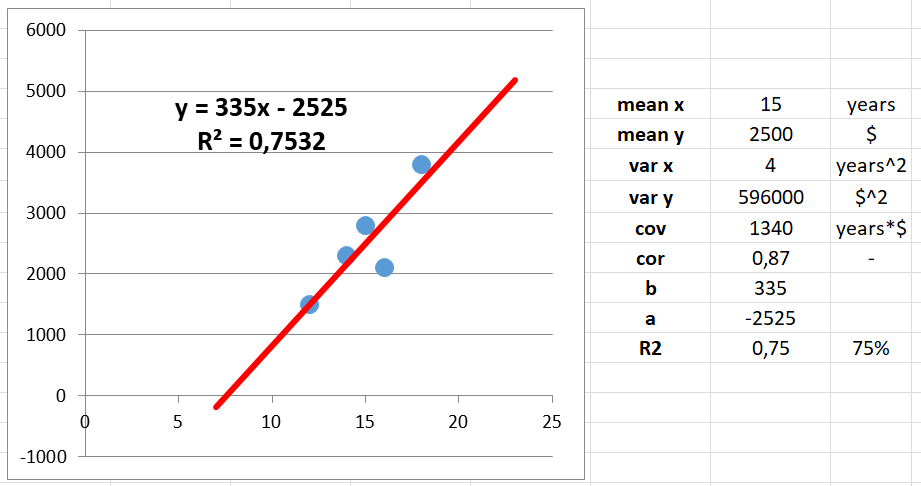
\includegraphics[width=\textwidth]{figs/example4}
\end{figure}
}


\frame<beamer>{\frametitle{\textcolor{CUNEFOrange}{Regression line: example}}
\begin{align*}
Y=-2525+335\cdot X
\end{align*}
\begin{itemize}
\item How does an increase in one year in education affect income?

\alert{For an increase in one year of education ($X$), income will increase by 335\$.}
\item What income would you predict for a person who has 17 years of education (12 years of high school + 5 years of double university degree)?

\alert{For a person who has had 17 years of education the predicted average income is 3170\$}.

\item Evaluate the goodness of fit.
\alert{$R^2$ has the value of 75\%, which indicates a good fit. In other words, the variable years of education ($X$) can explain 75\% of variation in the variable income ($Y$)}.
\end{itemize}
}

\section{Probability distributions: Normal and Student's \textit{t}}

\frame<beamer>{\frametitle{\textcolor{CUNEFOrange}{Normal distribution}}
\begin{itemize}
\item  By far the most popular and widely used of all continuous distributions is the \alert{Normal} (Gaussian, bell-shaped) distribution. 

\item It can take \textbf{any} value on the real  line, i.e.\ $-\infty,+\infty$.
 
\item Variables that are approximately Normally distributed: height, weight, shoe size, IQ, stock returns, average grades, log(income), etc.
 
\item In nature: snowflake sizes, temperatures, birth weights of any animal, etc.
 
\item Normal distribution is also the keystone of econometric and statistic theory, as it is the basis of the \alert{Central Limit Theorem}.
\end{itemize}
}


\frame<beamer>{\frametitle{\textcolor{CUNEFOrange}{Normal distribution}}
\begin{itemize}

\item If a r.v.\ $X$ is Normally distributed, i.e.\ $X\sim N(\mu, \sigma^2)$, then its PDF is given by:
\begin{align*}
f(x)=\frac{1}{\sqrt{2\pi\sigma^2}}\exp\left\{\frac{(x-\mu)^2}{2\sigma^2}\right\}
\end{align*}
\item The mean and variance are given by:
\begin{align*}
E[X]=\mu,\qquad V[X]=\sigma^2
\end{align*}
\end{itemize}
}


\frame<beamer>{\frametitle{\textcolor{CUNEFOrange}{Normal distribution}}
\begin{figure}
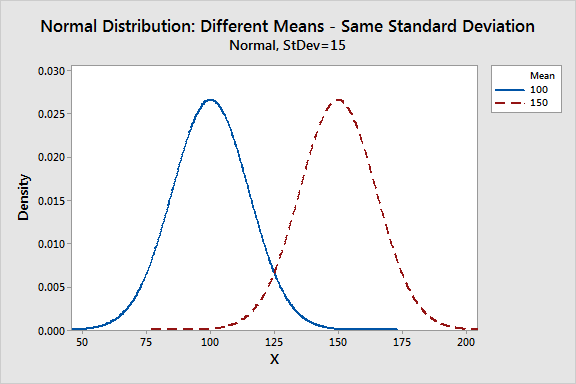
\includegraphics[width=0.48\textwidth]{figs/normal1}
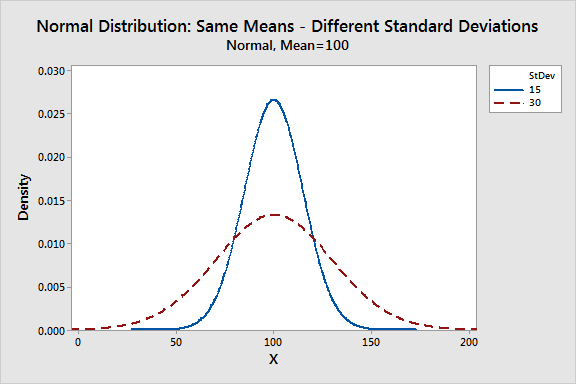
\includegraphics[width=0.48\textwidth]{figs/normal2}
\end{figure}
}


\frame<beamer>{\frametitle{\textcolor{CUNEFOrange}{Normal distribution: example}}

Call $X$ - students' height (in cm) at CUNEF. We assume it is Normally distributed $X\sim N(\mu=160,\sigma^2=100)$. What is the probability that a randomly selected student is shorter than 170cm?

\begin{figure}
\centering
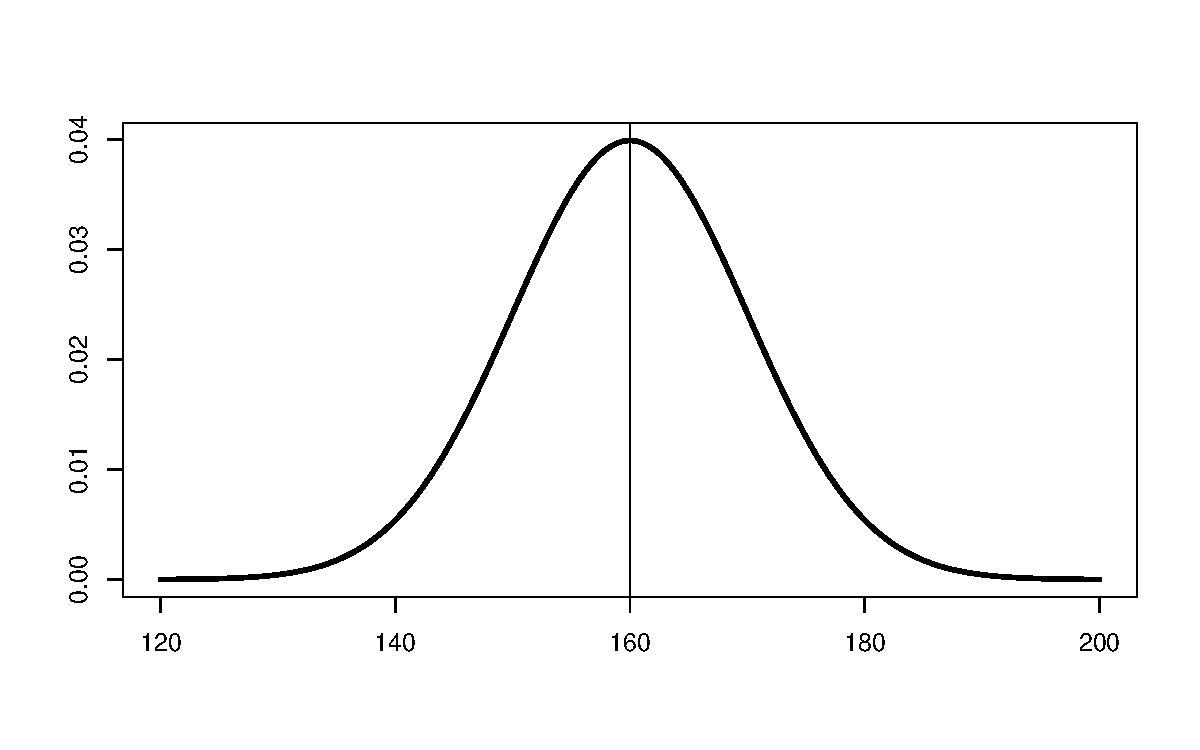
\includegraphics[width=0.8\textwidth]{figs/normheight}
\end{figure}
}


\frame<beamer>{\frametitle{\textcolor{CUNEFOrange}{Normal distribution: example}}

If $X\sim N(\mu=160,\sigma^2=100)$, then $P(X<170)$:

\begin{itemize}
\item Manually:
 \begin{align*}
P(X<170)=F(170)=\int_{-\infty}^{170} \frac{1}{\sqrt{2\pi\cdot 100}}\exp\left\{\frac{(x-160)^2}{2\cdot 100}\right\} dx=\alert{?}
\end{align*}

\item Use {\tt R: \alert{pnorm(170,160,sqrt(100))}}

\item Use \alert{statistical tables}.
\end{itemize}
}


\frame<beamer>{\frametitle{\textcolor{CUNEFOrange}{Normal distribution: statistical tables}}
\begin{itemize}
\item  Statistical tables facilitate the calculation of the complicated integrals:
\begin{align*}
P(X<x) = F(x)=\int_{-\infty}^x \frac{1}{\sqrt{2\pi\sigma^2}}\exp\left\{\frac{(x-\mu)^2}{2\sigma^2}\right\} dx
\end{align*}

\item But...  the statistical tables are calculated for \alert{standard} Normally distributed variables only: $X\sim N(0,1)$.
\end{itemize}
}


\frame<beamer>{\frametitle{\textcolor{CUNEFOrange}{Normal distribution: statistical tables}}
$X$ standard Normal  $X\sim N(0,1)$. What is the $P(X<0.75)$?
\begin{align*}
P(X<0.75)=F(0.75)=\int_{-\infty}^{0.75} \frac{1}{\sqrt{2\pi\cdot 1}}\exp\left\{\frac{(x-0)^2}{2\cdot 1}\right\} dx=0.7734
\end{align*}
\begin{figure}
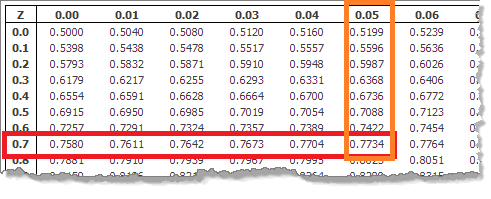
\includegraphics[width=0.7\textwidth]{figs/normal3.png}
\end{figure}
In { R: pnorm(0.75,0,1) = 0.7733726}
}

\frame<beamer>{\frametitle{\textcolor{CUNEFOrange}{Normal distribution: standardization }}
\begin{itemize}
\item And if the variable is \alert{not standard}  Normally distributed, we need to \alert{standardize} it first! And only then we can use the table.
\begin{align*}
Z=\frac{X-\mu}{\sigma}
\end{align*}
\item For example, $X$ is students' height (in cm) at CUNEF. We assume it is Normally distributed $X\sim N(\mu=160,\sigma^2=100)$. What is the probability that a randomly selected student is shorter than 170cm?
\begin{align*}
P(X<170)=P\left(\frac{X-\mu}{\sigma}<\frac{170-\mu}{\sigma} \right)=P\left(Z<\frac{170-160}{10} \right)=P(Z<1)
\end{align*}
\end{itemize}
}

\frame<beamer>{\frametitle{\textcolor{CUNEFOrange}{Normal distribution: standardization}}
Then $P(X<170)=P\left(\frac{X-\mu}{\sigma}<\frac{170-160}{10}\right)=P(Z<1)=0.8413$
\begin{figure}
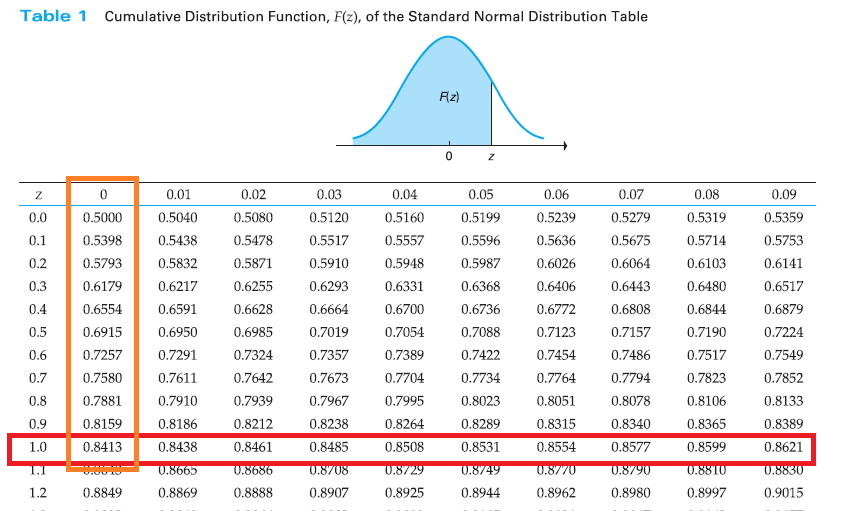
\includegraphics[width=0.8\textwidth]{figs/normal4}
\end{figure}
}

\begin{frame}{Student's $t$ distribution}
	
	
	\begin{itemize}			
		
		\item The Student's $t$ distribution is \alert{extremely popular distribution in statistics and in risk management}.
		
		\item was first described in English, in 1908, by William Sealy Gosset, an employee at the Guinness brewery in Dublin. 
		
		\item The probability density
		function can be written:
		\[
		f(x)=\frac{\Gamma\left(\frac{k+1}{2}\right)}{\sqrt{k \pi} \Gamma\left(\frac{k}{2}\right)}\left(1+\frac{x^{2}}{k}\right)^{-\frac{(k+1)}{2}},
		\]
		where $k$ is the degrees of freedom and $\Gamma$ is the gamma function.
		
	\end{itemize}
	
\end{frame}
%%%%%%%%%%%%%%%%%%%%%%%%%%%%%%%%%%%%%%%%%%%%%%%%%%%%%%%%%%%%%%%%%%%%
\begin{frame}{Student's $t$ distribution}
	
	
	\begin{itemize}			
		
		\item The $t$ distribution is symmetrical around its mean, which is equal to zero. For
		low values of $k$, the t distribution looks very similar to a standard normal distribution,
		except that it displays excess kurtosis. As $k$ increases, this excess kurtosis decreases.
		As $k$ approaches infinity, the $t$ distribution converges to a standard
		normal distribution.
				
	\end{itemize}

	\begin{figure}[h]
	\begin{center}
		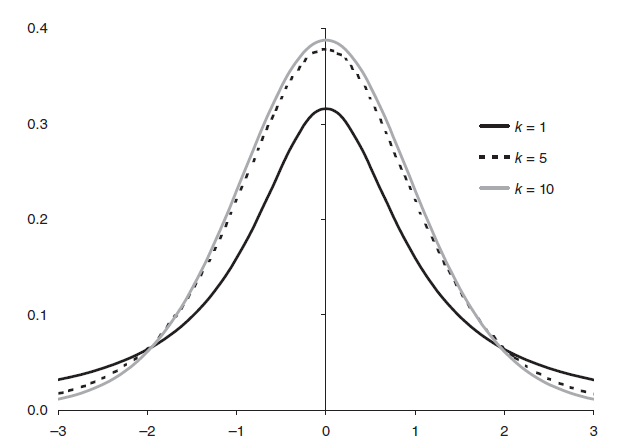
\includegraphics[width=0.55\linewidth]{figs/student.png}
	\end{center}
\end{figure}
	
\end{frame}
%%%%%%%%%%%%%%%%%%%%%%%%%%%%%%%%%%%%%%%%%%%%%%%%%%%%%%%%%%%%%%%%%%%%

\begin{frame}{Student's $t$ distribution}


	\begin{figure}[h]
	\begin{center}
		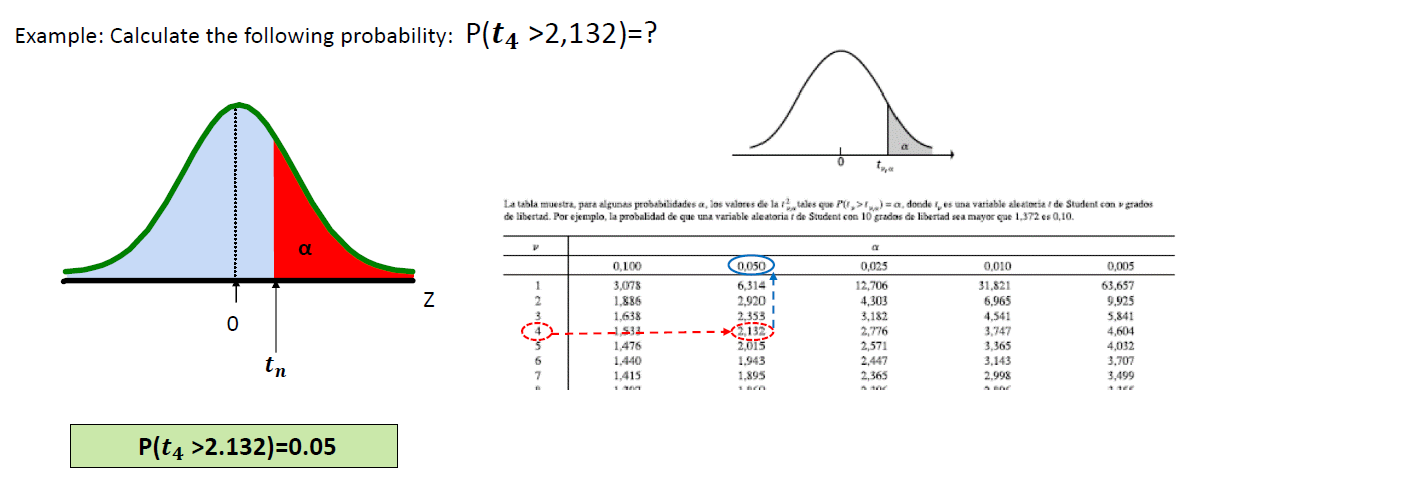
\includegraphics[width=1.25\linewidth]{figs/student_example.png}
	\end{center}
\end{figure}
	
\end{frame}
%%%%%%%%%%%%%%%%%%%%%%%%%%%%%%%%%%%%%%%%%%%%%%%%%%%%%%%%%%%%%%%%
\section{Point estimation}
\begin{frame}{Point estimation}
	
	
	\begin{itemize}
	\item Suppose we want to estimate the average income $\mu$ of all families in a city. 
 
 \item It seems logical to use the sample mean $\bar{X}$ as an estimator of the population mean $\mu$. 
 
 \item We need to select a random sample (for example $n=80$ ), and then we would obtain the average income of the sample, for example $\bar{x}=800$.

\item Then, the estimator of the population mean $\mu$ will be $\widehat{\mu}=\bar{X}$, that is, the mean statistic will be $\overline{\mathrm{X}}$ and the point estimate will be $\widehat{\boldsymbol{\mu}}=\overline{\boldsymbol{x}}=800$.

\item The problem is that there are many different ways to estimate the average income $\mu$. Using the sample mean $\bar X$ is only one of them. 
 
\item This makes it necessary to establish standards or criteria that allow choosing which is the ``best'' estimator among the possible ones in each case.
 
	\end{itemize}	
	
\end{frame}
%%%%%%%%%%%%%%%%%%%%%%%%%%%%%%%%%%%%%%%%%%%%%%%%%%%%%
\begin{frame}{Mean square error of the estimator}
	
	
	\begin{itemize}
	\item As the parameter is unknown, we will never know exactly to what extent each estimate (approximation) is far or close to the value of the parameter, that is, its use leads to the possibility of making a more or less high error when working with the point estimate as if it were the true value.

 \item We define the mean square error of the estimator $\hat{\theta}$, we denote as $\operatorname{MSE}(\hat{\theta})$, as the expected value of the square of the difference between the estimator $\hat{\theta}$ and the parameter $\theta$, that is
$$
\operatorname{MSE}(\hat{\theta})=\mathrm{E}\left[(\hat{\theta}-\theta)^2\right]
$$

\item The
smaller the error, the more accurate the estimate

 
	\end{itemize}	
	
\end{frame}
%%%%%%%%%%%%%%%%%%%%%%%%%%%%%%%%%%%%%%%%%%%%%%%%%%%%%
\begin{frame}{Mean square error of the estimator}
	
	
	\begin{itemize}
	\item An alternative expression of the mean squared error is:
\[
\text{MSE}(\hat{\theta}) = \mathbb{E}\left[(\hat{\theta} - \theta)^2\right] = \text{VAR}(\hat{\theta}) + (\underbrace{{\mathbb{E}[\hat{\theta}] - \theta}}_{\text{bias}[\hat{\theta}]})^2
\]

\item The MSE is equal to the variance of the estimator $\operatorname{VAR}(\hat{\theta})$, plus the square of the bias of the estimator: $E[\hat{\theta}]-\theta=\operatorname{bias}[\hat{\theta}]$.

\item Ideally, both quantities must be as small as possible, which is equivalent to the fact that the sampling distribution of $\hat{\theta}$  is concentrated around the value of the parameter $\theta$. The more concentrated, the lower the variance.
 
	\end{itemize}	
	
\end{frame}
%%%%%%%%%%%%%%%%%%%%%%%%%%%%%%%%%%%%%%%%%%%%%%%%%%%%%
\begin{frame}{Bias, efficiency, and consistency of an estimator}
	
	\begin{itemize}
 
	\item \textbf{Unbiased estimator}: $\hat{\theta}$ is an unbiased estimator of the parameter $\theta$ if the expectation of the estimator $\hat{\theta}$ is equal to the parameter $\theta$, that is:
$$
E[\hat{\theta}]=\theta
$$
Alternatively,
$$
\operatorname{bias}(\hat{\theta})=\mathrm{E}[\hat{\theta}]-\theta=0
$$
Otherwise we will say that the estimator is biased when $\operatorname{bias}(\hat{\theta})\ne 0$.

\item \textbf{Efficient estimator}: The most efficient estimator among a group of estimators will be the one with the smallest variance.

\item \textbf{Consistent estimator}: An estimator of a population $\theta$ is consistent when its variance tends to zero as $n$ increases.
$$
\lim _{n \rightarrow \infty} \operatorname{Var}(\widehat{\theta})=0
$$

 
	\end{itemize}	
	
\end{frame}
%%%%%%%%%%%%%%%%%%%%%%%%%%%%%%%%%%%%%%%%%%%%%%%%%%%%%

\section{Hypothesis tests}
\begin{frame}{Null  and Alternative Hypotheses}
	
	
	\begin{itemize}
	\item In this topic, we will review how to perform statistical tests to evaluate different hypotheses about a population.\medskip
	
	\item Our starting point will be the null hypothesis:
	$$
	\mathrm{H}_0: \mu=\mu_0 .
	$$
	
	\item In contrast the alternative hypothesis, $\mathrm{H}_1$, will take one of three forms, i.e. using $\neq,<$ or $>$, that is:
	$$
	\mathrm{H}_1: \mu \neq \mu_0 \quad \text { or } \quad \mathrm{H}_1: \mu<\mu_0 \quad \text { or } \quad \mathrm{H}_1: \mu>\mu_0
	$$
	Note that only one of these forms will be used per test. To determine which form to use will require careful consideration of the wording in the problem.
	\end{itemize}	
	
\end{frame}
%%%%%%%%%%%%%%%%%%%%%%%%%%%%%%%%%%%%%%%%%%%%%%%%%%%%%
\begin{frame}{Null and Alternative Hypotheses}
	
	
	\begin{itemize}
		
		\item \alert{How to correctly interpret a hypothesis test?}
		
		\item Remember that the problem is to use evidence in a randomly selected sample of data to decide whether to accept the null $H_{0}$ or to reject it in favor of the alternative $H_{1}$.
		
		\item If the null is accepted, \alert{this does not mean that the null can de declared ``true''}. 
		
		\item Rather, \alert{it is accepted tentatively} with the recognition that \alert{it might be rejected later based on additional evidence}.		
		
	\end{itemize}	
	
\end{frame}
%%%%%%%%%%%%%%%%%%%%%%%%%%%%%%%%%%%%%%%%%%%%%%%%%%%%%

\frame<beamer>{\frametitle{Tests for normal populations}
	
	\begin{itemize}
		
		
		\item Let us suppose that, having obtained sample data from a normal distribution, we use the estimator $\widehat{\theta}$ to estimate an unknown parameter $\theta$. \medskip
		
		\item Assume $\widehat{\theta}$ has the sampling distribution:
		$$
		\widehat{\theta} \sim N(\theta, V)
		$$
		where $V=\operatorname{Var}(\widehat{\theta})$ is assumed to be known. \medskip
		
		\item Hence the standard error, S.E. $(\widehat{\theta})$, is also known. 
		
		
	\end{itemize}		
	
	
}

\frame<beamer>{\frametitle{Tests for normal populations}

The hypothesis test would proceed using the following steps:

	\begin{itemize}
		
		
		\item 1. \alert{Define the hypotheses}. In this case suppose we test:
		$$
		\mathrm{H}_0: \theta=\theta_0 \quad \text { vs. } \quad \mathrm{H}_1: \theta>\theta_0 \text {. }
		$$
		
		\item 2. \alert{State the test statistic and its distribution}, then compute its value. We know that  standardization of $\widehat{\theta}$ yields:
		$$
		\frac{\widehat{\theta}-\theta_0}{\text { S.E. }(\widehat{\theta})} \sim N(0,1) .
		$$
		Next compute the test statistic value using the sample data, i.e. $\widehat{\theta}$ will be our point estimate of $\theta$.
		
		
	\end{itemize}		
	
	
}

\frame<beamer>{\frametitle{Tests for normal populations}
	

	
	\begin{itemize}
		
		
		\item 3. \alert{Define the critical region for a given significance level}, $\alpha$. For example, let $\alpha=0.05$, where $\alpha$ is the Type I error probability. Since we are conducting an upper-tailed test, we require $z_\alpha=z_{0.05}=1.645$, i.e. the $z$-value above which lies $5 \%$ probability.\medskip
		
		\item 4. \alert{Decide whether or not to reject $\mathrm{H}_0$}. If the test statistic value lies in the critical region then we will reject $\mathrm{H}_0$, otherwise we do not reject $\mathrm{H}_0$. 
		%A rejected $\mathrm{H}_0$ means the test is statistically significant at the specific significance level used. In the examination you will typically be required to test at two significance levels sequentially - more on this later.
		
		
		
	\end{itemize}		
\medskip
Remember that we will be always using a test statistic of the form:
$$
\frac{\text { point estimator - hypothesised value }}{\text { (estimated) standard error }} \text {. }
$$

Although this is not the format of all test statistics, it does cover a wide class of situations.
	
	
}
\frame<beamer>{\frametitle{$p$-values}
	
	\begin{itemize}
		
		
		\item So, given we reject $\mathrm{H}_0$ if the test statistic value is sufficiently extreme, we would also reject $\mathrm{H}_0$ if we obtained a sufficiently small $p$-value. \medskip
		
		\item To summarize, in the $p$-value world of testing, we use the following simple decision rule.\medskip
				
\begin{columns}
    \begin{column}{0.15\linewidth}
    \end{column}
    \begin{column}{0.7\linewidth}
        \begin{block}{$p$-value decision rule}
            \begin{itemize}
                \item Reject $\mathrm{H}_0$ if $p$-value $<\alpha$, where $\alpha$ is the significance level.
                \item Do not reject $\mathrm{H}_0$ if $p$-value $\geq \alpha$.
            \end{itemize}
        \end{block}
    \end{column}
    \begin{column}{0.15\linewidth}
    \end{column}
\end{columns}

		
		
	\end{itemize}
}


\frame<beamer>{\frametitle{Calculating $p$-values}
	
	
			
Let the test statistic value be $z$, and the test statistic (a random variable as it is constructed from an estimator) be $Z$. \medskip


Assuming a test statistic distribution which is symmetric about zero for the two-tailed test, in general these can be summarized as follows.\medskip

\begin{table}
	\begin{center}
		\begin{tabular}{c|c} 
			Form of $\mathrm{H}_1$ & $p$-value calculation \\
			\hline $\mathrm{H}_1: \theta \neq \theta_0$ & $2 \times P(Z \geq|z|)$ \\
			$\mathrm{H}_1: \theta<\theta_0$ & $P(Z \leq z)$ \\
			$\mathrm{H}_1: \theta>\theta_0$ & $P(Z \geq z)$
		\end{tabular}
	\end{center}
\end{table}
				
			
}





%%%%%%%%%%%%%%%%%%%%%%%%%%%%%%%%%%%%%%%%%%%%%%%%%%%%%

%%%%%%%%%%%%%%%%%%%%%
% Back Page
%%%%%%%%%%%%%%%%%%%%
\NoLogoFootline
{\usebackgroundtemplate{%

\includegraphics[width=\paperwidth,height=\paperheight]{figs/back_page.png}}
\slide{}{}}


\end{document}


